% --- Template for thesis / report with tktltiki2 class ---
% 
% last updated 2013/02/15 for tkltiki2 v1.02

\documentclass[english]{tktltiki2}

% tktltiki2 automatically loads babel, so you can simply
% give the language parameter (e.g. finnish, swedish, english, british) as
% a parameter for the class: \documentclass[finnish]{tktltiki2}.
% The information on title and abstract is generated automatically depending on
% the language, see below if you need to change any of these manually.
% 
% Class options:
% - grading                 -- Print labels for grading information on the front page.
% - disablelastpagecounter  -- Disables the automatic generation of page number information
%                              in the abstract. See also \numberofpagesinformation{} command below.
%
% The class also respects the following options of article class:
                       %   10pt, 11pt, 12pt, final, draft, oneside, twoside,
%   openright, openany, onecolumn, twocolumn, leqno, fleqn
%
% The default font size is 11pt. The paper size used is A4, other sizes are not supported.
%
% rubber: module pdftex

% --- General packages ---

\usepackage[utf8]{inputenc}
\usepackage[T1]{fontenc}
\usepackage{lmodern}
\usepackage{microtype}
\usepackage{amsfonts,amsmath,amssymb,amsthm,booktabs,color,enumitem,graphicx}
\usepackage[pdftex,hidelinks]{hyperref}



% Automatically set the PDF metadata fields
\makeatletter
\AtBeginDocument{\hypersetup{pdftitle = {\@title}, pdfauthor = {\@author}}}
\makeatother

% --- Language-related settings ---
%
% these should be modified according to your language

% babelbib for non-english bibliography using bibtex
\usepackage[fixlanguage]{babelbib}
\selectbiblanguage{english}

% add bibliography to the table of contents
\usepackage[nottoc]{tocbibind}
% tocbibind renames the bibliography, use the following to change it back
\settocbibname{Sources}

% --- Theorem environment definitions ---

\newtheorem{lau}{Lause}
\newtheorem{lem}[lau]{Lemma}
\newtheorem{kor}[lau]{Korollaari}

\theoremstyle{definition}
\newtheorem{maar}[lau]{Määritelmä}
\newtheorem{ong}{Ongelma}
\newtheorem{alg}[lau]{Algoritmi}
\newtheorem{esim}[lau]{Esimerkki}

\theoremstyle{remark}
\newtheorem*{huom}{Huomautus}


% --- tktltiki2 options ---
%
% The following commands define the information used to generate title and
% abstract pages. The following entries should be always specified:

\title{Comparison of Virtualization Techniques in Distributed Cloud Environments}
\author{Lauri Suomalainen}
\date{\today}
\level{Master's Thesis}
\abstract{Abstract}

% The following can be used to specify keywords and classification of the paper:

\keywords{Virtualization, Distributed Systems, Containerization}

% classification according to ACM Computing Classification System (http://www.acm.org/about/class/)
% This is probably mostly relevant for computer scientists
% uncomment the following; contents of \classification will be printed under the abstract with a title
% "ACM Computing Classification System (CCS):"
% \classification{}

% If the automatic page number counting is not working as desired in your case,
% uncomment the following to manually set the number of pages displayed in the abstract page:
%
% \numberofpagesinformation{16 sivua + 10 sivua liitteissä}
%
% If you are not a computer scientist, you will want to uncomment the following by hand and specify
% your department, faculty and subject by hand:
%
% \faculty{Matemaattis-luonnontieteellinen}
% \department{Tietojenkäsittelytieteen laitos}
% \subject{Tietojenkäsittelytiede}
%
% If you are not from the University of Helsinki, then you will most likely want to set these also:
%
% \university{Helsingin Yliopisto}
% \universitylong{HELSINGIN YLIOPISTO --- HELSINGFORS UNIVERSITET --- UNIVERSITY OF HELSINKI} % displayed on the top of the abstract page
% \city{Helsinki}
%


\begin{document}

% --- Front matter ---

\frontmatter      % roman page numbering for front matter

\maketitle        % title page
\makeabstract     % abstract page

\tableofcontents  % table of contents

% --- Main matter ---

\mainmatter       % clear page, start arabic page numbering

\section{Introduction}

Cloud adoption is growing ever so fast with vast majority of both enterprises and small and medium businesses leveraging on cloud computing one way or another.\cite{stateofthecloud} While private cloud usage is growing at steady pace, its growth is eclipsed by that of public cloud usage which is estimated to grow trice as fast when compared to private clouds. 
Contributing to the accelerated speed of cloud adoption is the trend of simultaneous use of multiple cloud environments and services, both private and public. The concept of using multiple clouds to support and enable same business is called \textit{Hybrid cloud} and on average enterprises report using and experimenting with almost five different clouds simultaneously. 
Another trend of cloud computing is a shift away from virtualised clouds to running workloads directly on hardware. This \textit  {bare-metal computing} interests companies running computationally heavy workloads such as Big Data and Machine learning as bare-metal seeks to amend performance overheads inherent to virtualisation. Openstack Foundation report a stark increase in the usage of its bare-metal service \textit{Ironic} \cite{openstacksurvey} and along with the possibility to use bare-metal servers with major public cloud providers there are also relatively new service providers such as \textit{Vultr} \cite{vultr} and \textit{Packet} \cite{packet} who focus especially on providing bare-metal servers as a service.

Growing usage of both hybrid clouds and the variety of the underlying hardware and interfaces to use them introduce complexity to management of these systems. As a natural reaction, there are now many tools to abstract and manage this complexity. For example, IBM has their own tool \textit{IBM Multicloud Manager} \cite{ibmmulticloud} and \textit{Rancher} \cite{rancher} has been a popular framework for handling multiple Kubernetes clusters \cite{Kubernetes}. This thesis focuses on \textit{Cloudify} \cite{cloudify} which is also a tool to manage multiple clouds. What sets it apart from others however is the fact that it aims to be a general tool independent of the underlying platform implementations meaning that the user can control multiple clouds and even single physical machines as a generic set of resources without extensive knowledge of their implementation. This opens up avenues in optimising cloud resource usage and introducing hardware that has not traditionally been used as cloud computing resources such as consumer-grade computers and single-board computers such as Raspberry PIs. However, as bare-metal cloud computing is not as popular as applications of virtualised computing resources, Cloudify's bare-metal capabilities remain underdeveloped.

In this thesis I identify shortcomings related to Cloudify's capability of managing generic computational resources such, as consumer-grade computers, and provide prototypical solutions addressing them. Main problems addressed are Cloudify's inability to automatically detect and manage physical hosts in the cluster and its lacking knowledge of the performance capabilities of the said hosts. My key contributions are:

\begin{enumerate}
\item  A software solution which detects joining and parting hosts in the cluster network automatically without a need for human intervention and provides them to the Cloudify Manager for allocation.
\item A modification to Cloudify's Host-pool service so that it retrieves and stores hardware data and performance capabilities of the hosts. In the future Cloudify Manager can use this data to optimise resource usage and make more intelligent workload allocation choices.
\end{enumerate}

Both of the solutions integrate seamlessly with the existing Cloudify components. I also perform experiments on real machines to showcase and validate the capabilities and correctness of my solutions within the scope of this thesis. The features I am addressing are lacking likely because Cloudify's develpment team's focus has been on integrations with the major cloud platforms and generic hardware provisioning is a niche use case compared to them.

The remainder of this thesis is structured as follows: First in section~\ref{background} I give a background overview of common cloud computing concepts. Then I follow with the background review of Cloudify, comparing it conceptually to OpenStack which serves as an example of a typical Cloud computing platform. I also provide a quick overview of hybrid cloud and bare-metal management tools similar to Cloudify.
From section~\ref{systemdesign_and_implementation} onwards I focus on identifying the scope of the prototype and the shortcomings of Cloudify I set out to correct. I provide an overview of the parts in Cloudify with which my proposed system interacts with and detail a high level design of my solutions for automating host detection and retrieval and storage of hardware data. Section~\ref{technical_implementation} presents the lower level details of solutions' implementation followed by the experiments in section~\ref{experiments} showcasing and validating the solutions' capabilities. Finally in chapter~\ref{future} I review future work and research required to fully develop the system beyond the prototype.

Both solutions, Discovery Service and Modified Host-pool Service, presented in this thesis are open source and can be found at \url{https://bitbucket.org/Fleuri/discoveryserviceforcloudify/src/master/}  and \url{https://github.com/Fleuri/cloudify-host-pool-service} respectively.

\pagebreak
\section{Background}

			In cloud computing, there are multiple recognised service models which dictate how the users can use the given system and what privileges they are given \cite{Mell:2011:SND:2206223}. In its most limited form, a cloud service is offered to user as a predefined application or a set of applications. The users has some interface for interacting with the applications but is given no control over anything else such as other applications, the operating system the application is running on or network and hardware configurations. This is generally known as Software as a Service or SaaS for short. The most permissible service model is known as IaaS, Infrastructure as a Service. In its archetype the user gets access to all fundamental computing resources, possibly including some network components, and can run arbitrary software including operating systems. The user experience should be similar to that with their personal computers. The user is not allowed to access the underlying cloud infrastructure. Between the two falls Platform as a Service (PaaS). PaaS typically allows user to deploy their own applications along with their dependent libraries, tools, services etc. provided that they are supported by the cloud provider. The user has no control over underlying cloud infrastructure, operating system, storage or network but usually can configure certain settings and possibly choose different supporting services the cloud provider offers. There are also other "aaS" such as Data as a Service (DaaS) and Storage as a Service (SaaS) but they are based on one of the three aforementioned service models or are variations or subsets of them. Sometimes the numerous models are referenced with umbrella terms of XaaS and EaaS meaning Everything as a Service for both or Anything as a Service for the former \cite{XaaS}.

Virtualisation in the context of distributed cloud environments usually refers to virtual machines. The core idea is analogous to computer hardware virtualisation. Operating systems offer an interface for the processes to utilise the computer hardware while giving them an illusion that they have all of the hardware for themselves \cite{ArpaciDusseau14-Book}. In reality the resources are shared among many processes. Likewise in cloud environments resources are being share by processes but also by different users running different operating systems, configurations and programs. As with the processes, users are given an impression that they alone have access to the underlying hardware resources, whereas in reality there are multiple users using the same physical machines.


There are several reasons as to why would one prefer a virtualised environment to a non-virtualised one. Obviously in multitenant cloud services it is crucial for the service provider to maximise the use of their hardware resources. Thus it is imperative for the provider to try to share the limited hardware resources among as many users' virtualised environments as possible. Otherwise every user would need their own physical machine in the system which would both require more resources per user and leave resources underused. From the fault tolerance perspective, using virtual machines in a distributed environment decreases their dependency on the underlying physical hardware \cite{Clark05livemigration}. That is because in virtual machine architectures which support live migration of operating system instances can be seamlessly moved from one physical machine to another. This also helps the load-balancing in the distributed system and allows low-level and physical maintenance of the hardware without considerably disrupting the usage of the system. A end-user also has many reasons to use virtualised cloud services. User only needs a lightweight computer with an internet connection to perform computationally challenging tasks in the cloud back-end. Similarly devices with little storage capacity can leverage from a cloud service's vast storage space. Some users would like to use applications and programs not native to their operating system of choice making another virtualised OS a convenient option \cite{ArpaciDusseau14-Book}. Virtualised environment allows software developers to test and debug their software with many different settings, as virtualised environments can have different operating systems and available hardware resources. Naturally this also allows emulating completely different devices \cite{eder2016hypervisor}.

\subsection{Heterogeneous clouds, bare-metal and hybrid}

One of the most common assumptions of the current cloud computing paradigm is that the cloud environment is built on commodity hardware \cite{Heterogeneous}. Even if that was not the case, virtualisation and orchestration techniques more often than not abstract the underlying hardware making it invisible to users. Naturally, this can cause problems if the cluster's devices' capabilities differ from each other drastically. In a multitenant cloud the use cases, workloads and resource needs differ between users, but the cloud is only capable of offering generic solutions for everyone. 

Other motivations to deploy heterogeneous hardware to data centres relating to different use cases and needs stem from bare-metal solutions and green computing movement \cite{Kurp2008}. For example, if a user is running mainly computationally light applications that perhaps only run for a short time, it is wasteful to keep full-fledged rack servers running if the same task could be accomplished with hardware requiring less power and outputting less heat and e.g. a Raspberry PI \cite{raspberry}. In addition, such machines are magnitudes cheaper than traditional rack servers. Virtualisation techniques deployed in current clouds have wide range of benefits but they incur overheads making them undesirable for certain high-performance computing tasks like Big Data analysis and graphical processing. Such tasks may also require specialised hardware to optimise the performance and thus in the best scenario user should have information of the hardware capabilities and be able to control on which nodes their tasks are run.

Ability to know and control nodes and their capabilities are also relevant in the so-called \textit{hybrid clouds}. One way to classify different clouds is by which party offers the service. Clouds hosted by an organisation meant for its internal used are referred to as \textit{Private clouds} whereas cloud service offered by an organisation for other party to rent and use is known as \textit{Public clouds} \cite{cloudcomputingconcepts}. Hybrid cloud is as the name suggests a combination of these two. An organisation may need to provision resources from a public cloud occasionally for different use-cases and workloads to complement their own environment or the private cloud is used to control data more securely as the service using the data is offered in a public cloud. Use cases and motivations for deploying a hybrid cloud vary, but a result is most likely a cluster with heterogeneous hardware.


	

\subsection{Virtualisation Techniques}

Traditionally virtualisation has referred to a software abstraction layer residing between the computer hardware and the operating system. \cite{taxonomy} This layer has been called Virtual Machine Monitor (VMM) or more recently a hypervisor and it hides and abstracts the computing resources from the OS, allowing multiple OSs to run simultaneously on the same hardware. There are multiple ways to run hypervisor-based virtualisation. Lately a technology called container-based virtualisation has been gaining popularity. Instead of emulating whole hardware, containers make use of features provided by the host operating system to isolate processes from each other and other containers \cite{eder2016hypervisor}.

\subsubsection{Full virtualisation}

In full virtualisation, the hypervisor runs on top of the host OS. The guest OSs run on top of the hypervisor which in turn emulates the underlying real hardware to them. The hypervisors running on top of the host OS are generally referred as \textit{Type 2 Hypervisors} \cite{eder2016hypervisor}. The guest OSs can be arbitrary. Figure ~\ref{fig:full} shows the full virtualisation architecture with the hypervisor running on top of the Host OS and Guest OSs on top of the hypervisor using their emulated hardware. 

\begin{figure}[ht!]
\centering
  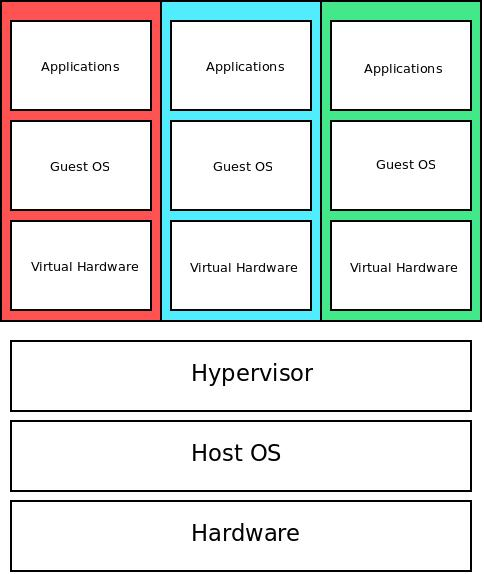
\includegraphics[width=10cm,height=10cm, keepaspectratio]{fullvirt.jpeg}%
  \caption{Full virtualisation architecture}
  \label{fig:full}
\end{figure}

The main advantage of full virtualisation is that it is easy to deploy and should not pose problems to an average user but the virtualisation overhead results in significantly reduced performance when compared to running directly on hardware. Popular examples of full virtualisation applications are Oracle's \textit{VirtualBox}\cite{VirtualBox} and \textit{VMware Workstation}\cite{WorkStation}. 

\subsubsection{Hardware-Layer virtualisation}

Hardware-Layer virtualisation is also a type of full virtualisation, but unlike Type 2 hypervisors, the so called \textit{Type 1 Hypervisors} (also \textit{native} and \textit{bare metal}) run directly on hardware. As seen on figure ~\ref{fig:hardware} there's no Host OS per se. Instead the Guest OSs access to hardware resources is controlled by the hypervisor.

\begin{figure}[ht!]
\centering
  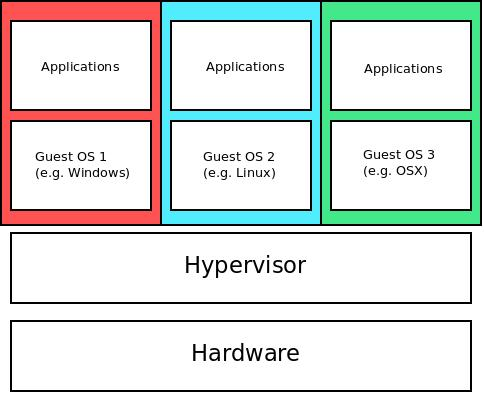
\includegraphics[width=10cm,height=10cm, keepaspectratio]{hwlayer.jpeg}%
  \caption{Hardware-Layer virtualisation architecture}
  \label{fig:hardware}
\end{figure}

Running directly on hardware, Hardware-Layer virtualisation techniques suffer less performance overhead than their OS-layer counterparts. On the other hand, Type 2 hypervisors being essentially applications themselves can be ran in parallel on the host OS whereas Type 1 hypervisors can not. For an average user, setting up a Type 1 hypervisor can be more difficult than Type 2. Commercial examples of Type 1 Hypervisors include Microsoft's \textit{Hyper-V}\cite{hyperv} and VMware's \textit{VSphere} \cite{vsphere}.

\subsubsection{Container-based virtualisation}

Instead of virtualising the underlying hardware, container-based virtualisation also known as OS-Layer virtualisation \cite{taxonomy} focuses on user space and allows running multiple operating systems in parallel as applications using the same kernel as the host operating system. A prime example of a popular container-based virtualisation platform is \textit{Docker} \cite{docker} which leverages on native Linux kernel features to virtualise and isolate OS instances. Figure ~\ref{fig:container} shows a container-based virtualisation architecture in which containerised environments are running operating systems on host OS's kernel. 

\begin{figure}[ht!]
\centering
  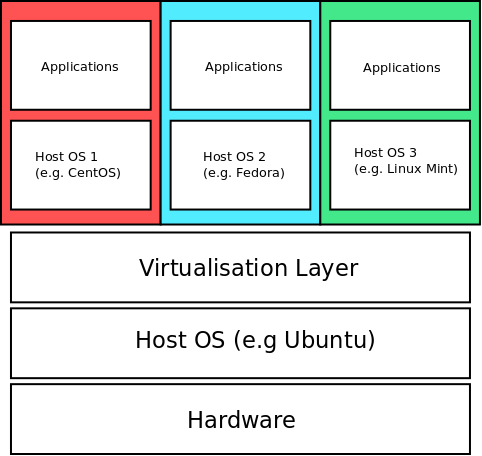
\includegraphics[width=10cm,height=10cm, keepaspectratio]{containers.png}%
  \caption{Container-based architecture}
  \label{fig:container}
\end{figure}

Container-based virtualisation does not need to emulate the hardware as containers communicate directly with the host kernel \cite{eder2016hypervisor} and are thus very fast to start. They also do not require all of the components a fully virtualised environment would need to run and therefore their resource fingerprint is minimal when compared to hypervisor-based virtualisation techniques. \linebreak
The obvious drawback of the technique is that the kernel of the virtualised OS has to be the same as that of Host OS e.g. In a situation depicted in figure ~\ref{fig:container} operating systems based on  Linux kernel could be ran on Ubuntu Host OS but OSs like Windows or OSX could not. On certain virtualisation platforms resource-intensive containers can also affect other containers detrimentally as the shared host OS's kernel is forced to spend its execution time on handling the instructions from the stressed container \cite{Xaviercontainer}.


\subsubsection{Paravirtualisation}

Paravirtualisation differs from full virtualisation by requiring the Guest OS to be modified in order to accomodate the virtual environment in which it is ran. Otherwise the architecture is similar to that of full virtualisation, but with thinner hypervisor allowing performance close to that of a non-virtualised environment. A well-known example of a paravirtualisation hypervisor is \textit{Xen}\cite{xen}.

\subsubsection{Unikernels}

Unikernels are a relatively recent take on virtualising services. Building on the notion that in cloud environments each VM usually specialises to provide only one service even if each VM contains a full-fledged general computer \cite{unikernels}. Unikernels are essentially minimal single-purpose library operating system (\textit{LibOS})\cite{libos} VMs with a single address space. They contain only the minimal set of services, implemented as libraries, built and sealed against modification to run the one application. Unlike the earlier LibOSes unikernels do not require a host OS to run but run directly on a VM hypervisor, such as Xen.

Some benefits of unikernels are obvious. Constructing VMs with minimal set of service libraries results in small images and resource footprints as well as fast boot times. Other benefits include reduced attack surface due to smaller codebase and sealing preventing any code not compiled during the creation of the VM from running. Single-address space improves context switching and eliminates the need for privilege transitions making system calls as efficient as function calls \cite{osv}. Running directly on the hypervisor instead of a host OS eliminates superfluous levels of hardware abstraction.

Optimisation and simplification are not without drawbacks. By definition, unikernels are not intended for general-purpose multi-user computing but for microservice cloud environments. Running multiple applications on a single VM is risky due single-address space does not offer any inherent resource isolation. As unikernels are sealed during compiling, it is not possible to do changes to them afterwards. User is instead required to compile and launch a completely new modified VM.

Popular examples of unikernels are \textit{MirageOS}\cite{mirage} and \textit{OSv}\cite{osv}.

\subsection{Experiment technologies}

This section discusses the technologies used and studied in the experiment in more detail. Virtualisation technologies are Docker, Xen, KVM and OSv and they are run on an OpenStack testbed.

\subsubsection{Docker}


\subsubsection{Xen}
\subsubsection{KVM}
\subsubsection{OSv}


\section{System design and implementation}
\section{Experiments and measurements}
\section{Related work}
\section{Future research}
\section{Conclusions}




% --- References ---
%
% bibtex is used to generate the bibliography. The babplain style
% will generate numeric references (e.g. [1]) appropriate for theoretical
% computer science. If you need alphanumeric references (e.g [Tur90]), use
%
% \bibliographystyle{babalpha-lf}
%
% instead.

\bibliographystyle{babplain-lf}
\bibliography{references-en}


% --- Appendices ---

% uncomment the following

% \newpage
% \appendix
% 
% \section{Esimerkkiliite}

\end{document}